\documentclass[12pt,a4paper]{article}
%%%%%%%%%%%%%%%%%%%%%%%%%%%%%%%%%%%%%%%%%%%%%%%%%%%%%%%%%%%%%%%%%%%%%%%%%%%%%%%%
%%%%%%%%%%%%%%%%%%%%%%%%%%%%%%%%%%%%%%%%%%%%%%%%%%%%%%%%%%%%%%%%%%%%%%%%%%%%%%%%
%%% Template for AIMS Rwanda Assignments         %%%              %%%
%%% Author:   AIMS Rwanda tutors                             %%%   ###        %%%
%%% Email: tutors2017-18@aims.ac.rw                               %%%   ###        %%%
%%% Copyright: This template was designed to be used for    %%% #######      %%%
%%% the assignments at AIMS Rwanda during the academic year %%%   ###        %%%
%%% 2017-2018.                                              %%%   #########  %%%
%%% You are free to alter any part of this document for     %%%   ###   ###  %%%
%%% yourself and for distribution.                          %%%   ###   ###  %%%
%%%                                                         %%%              %%%
%%%%%%%%%%%%%%%%%%%%%%%%%%%%%%%%%%%%%%%%%%%%%%%%%%%%%%%%%%%%%%%%%%%%%%%%%%%%%%%%
%%%%%%%%%%%%%%%%%%%%%%%%%%%%%%%%%%%%%%%%%%%%%%%%%%%%%%%%%%%%%%%%%%%%%%%%%%%%%%%%


%%%%%% Ensure that you do not write the questions before each of the solutions because it is not necessary. %%%%%% 


%%%%%%%%%%%%%%%%%%%%%%%%% packages %%%%%%%%%%%%%%%%%%%%%%%%
\usepackage{amsmath}
\usepackage{amssymb}
\usepackage{placeins}
\usepackage{amsthm}
\usepackage{amsfonts}
\usepackage{graphicx}
\usepackage[all]{xy}
\usepackage{tikz}
\usepackage{verbatim}
\usepackage{float}
\usepackage{bbm} %indicator function 1 package
\usepackage{bbold} %indicator function 1 package with bold
\usepackage[left=2cm,right=2cm,top=3cm,bottom=2.5cm]{geometry}
\usepackage{hyperref}
\usepackage{caption}
\usepackage{subcaption}
\usepackage{psfrag}
\usepackage{mathrsfs}

%%%%%%%%%%%%%%%%%%%%% students data %%%%%%%%%%%%%%%%%%%%%%%%
\newcommand{\student}{Yusuf Brima}
\newcommand{\course}{Quantitative Methods in Gene Expression}
\newcommand{\assignment}{1}

%%%%%%%%%%%%%%%%%%% using theorem style %%%%%%%%%%%%%%%%%%%%
\newtheorem{thm}{Theorem}
\newtheorem{lem}[thm]{Lemma}
\newtheorem{defn}[thm]{Definition}
\newtheorem{exa}[thm]{Example}
\newtheorem{rem}[thm]{Remark}
\newtheorem{coro}[thm]{Corollary}
\newtheorem{quest}{Question}[section]

%%%%%%%%%%%%%%  Shortcut for usual set of numbers  %%%%%%%%%%%

\newcommand{\N}{\mathbb{N}}
\newcommand{\Z}{\mathbb{Z}}
\newcommand{\Q}{\mathbb{Q}}
\newcommand{\R}{\mathbb{R}}
\newcommand{\C}{\mathbb{C}}

%%%%%%%%%%%%%%%%%%%%%%%%%%%%%%%%%%%%%%%%%%%%%%%%%%%%%%%555
\begin{document}

%%%%%%%%%%%%%%%%%%%%%%% title page %%%%%%%%%%%%%%%%%%%%%%%%%%
\thispagestyle{empty}
%\begin{figure}
%    \centering
%    \includegraphics[width=\textwidth]{aims_rwanda.jpg}
%\end{figure}
\begin{center}
\textbf{AFRICAN INSTITUTE FOR MATHEMATICAL SCIENCES \\[0.5cm]
(AIMS RWANDA, KIGALI)}
\vspace{1.0cm}
\end{center}

%%%%%%%%%%%%%%%%%%%%% assignment information %%%%%%%%%%%%%%%%
\noindent
\rule{17cm}{0.2cm}\\[0.3cm]
Name: \student \hfill Assignment Number: \assignment\\[0.1cm]
Course: \course \hfill Date: \today\\
\rule{17cm}{0.05cm}
\vspace{1.0cm}

\section*{Question 1}
 Gene expression is controlled by two regulators  that turn the operon "on" and "off" in response to lactose and glucose levels: the lac repressor and Catabolite Activator Protein (CAP). The lac repressor acts as a lactose sensor. It normally blocks transcription of the operon, but stops acting as a repressor when lactose is present. The lac repressor senses lactose indirectly, through its isomer allolactose where Catabolite Activator Protein (CAP) acts as a glucose sensor.  It activates transcription of the operon, but only when glucose levels are low. CAP senses glucose indirectly,  through the hunger signal molecule cAMP.  In the presence of lactose and glucose, allolactose binds the Repressor to allow RNA Polymerase to transcribe gene to mRNA.
In this simple model,  we suppose that the production of mRNA is constant which give rise to the following differential equation \eqref{eq:1}
\begin{equation}
\frac{dM}{dt} = M_0 - \lambda M 
\label{eq:1}
\end{equation}

Where \\
$ M_0=  $  is the constant production of mRNA in the absence of protein,\\
$ M=  $  is the concentration of mRNA\\
and $ \lambda = $ turnover rate of mRNA.
\section*{Question 2 }
if we suppose that this gene is introduced into a newly replicated cell  that did not yet have any gene X mRNA we get the following differential equation \eqref{eq:2}
\begin{equation}
\frac{dM}{dt} = M_0
\label{eq:2}
\end{equation}
From \eqref{eq:2} equation,  we observe that $mRNA$ is non-existent.   By using Separation of Variables, we solve \eqref{eq:2} as follows:

\begin{eqnarray*}
\frac{dM}{dt} &=& M_0\\
\int dM &=& \int M_0 dt\\
M &=& M_0t + c
\end{eqnarray*}

At $t=0 \implies   M=0$.  So at time $t=0$,  no production of mRNA,  therrefore, we obtain the following graph:
\begin{figure}[H]
\centering
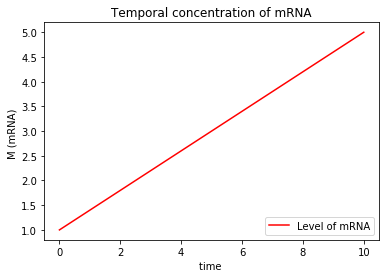
\includegraphics[scale=0.5]{./gaphics/q_2.png}
\caption{ }
\end{figure}

\section*{Question 3}
The differential equation that captures the level of protein P encoded by gene X,
where the synthesis of P depends on concentrations of M as well as a term that accounts for
turnover of existing P in the cell is modeled by the following differential equation in \eqref{eq:3}.
\begin{equation}
\frac{dP}{dt} =   \alpha M - \gamma_p P
\label{eq:3}
\end{equation}
where \\
$\alpha = $   translation rate\\
$ \gamma_p =  $ turnover rate of existing P\\
 $P = $ concentration of protein
\section*{Question 4}
When we consider the scenario where $M$ is lacking,  we get:
\begin{equation}
\frac{dP}{dt} = -\gamma_p P
\label{eq:4}
\end{equation}
And in the scenario  where P is lacking,  we obtain:

\begin{equation}
\frac{dP}{dt} = \alpha M 
\label{eq:4}
\end{equation}
\begin{align*}
\frac{dP}{dt} &=  0
\end{align*}
This indicates the lack of both mRNA and protein,  and the graph of the Ordinary Differential Equations solution is plotted below.
\begin{figure*}[th!]
    \centering
    \begin{subfigure}[t]{0.5\textwidth}
        \centering
        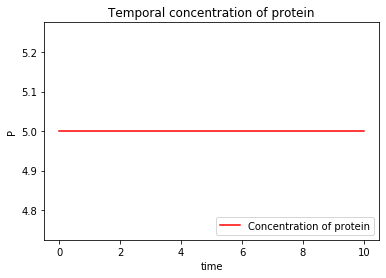
\includegraphics[height=1.8in]{./gaphics/q_4a.png}
        %\caption{}
    \end{subfigure}%
    ~ 
    \begin{subfigure}[t]{0.5\textwidth}
        \centering
        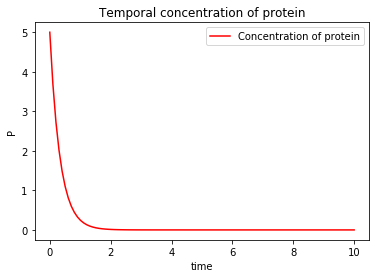
\includegraphics[height=1.8in]{./gaphics/q_4b.png}
        %\caption{}
    \end{subfigure}
    \caption{}
\end{figure*}
\section*{Question 5}
The differential equations to  show
how the levels of $M$ and $P$ would change with time, and with respect to each other is as follows:
\begin{equation}
  \frac{dM}{dt} = M_0 -  \lambda M 
  \label{eq:5}
\end{equation} 

\begin{equation}
  \frac{dP}{dt} = \alpha M - \gamma_p P
  \label{eq:6}
\end{equation}
The  plotted graph showing two overlapping curves and another graph showing level of $P$ and $M$.
\begin{figure*}[th!]
    \centering
    \begin{subfigure}[t]{0.5\textwidth}
        \centering
        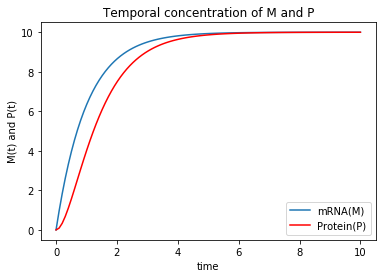
\includegraphics[height=1.8in]{./gaphics/q_5a.png}
        %\caption{}
    \end{subfigure}%
    ~ 
    \begin{subfigure}[t]{0.5\textwidth}
        \centering
        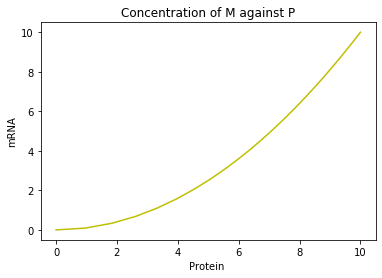
\includegraphics[height=1.8in]{./gaphics/q_5b.png}
        %\caption{}
    \end{subfigure}
   \caption{}
\end{figure*}

\section*{Question 6}
In Molecular Biology: half life is defined as the time taken for a radioactive substance to decay to halve the original quantity.


If we consider a mutation that affects the structure of the mRNA so that it becomes very unstable,  thereby the mRNA half-lives for a bacterial cell. This phenomenon is modeled on the impact would be on the $M$ and $P$  in equation  \eqref{eq:7}.

\begin{equation}
 M\left(  \frac{t}{2} \right) = \frac{\alpha}{\gamma} + ce^{- \frac{\gamma t}{2}}
 \label{eq:7}
\end{equation}
Below is the curve showing the impact on $M$ and$ P$:
\begin{figure}[H]
\centering
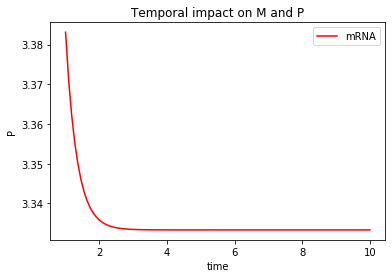
\includegraphics[scale=0.5]{./gaphics/q_6.png}
\caption{ }
\end{figure}
\section*{Question 7}
Considering a mutation that greatly stabilizes the protein $P$,  but otherwise has no impact on
transcription or translation – is presented in equations .
\begin{equation}
\frac{dM}{dt} =  M_0 -  \lambda M 
\label{eq:8}
\end{equation}
\begin{equation}
\frac{dP}{dt} =  \alpha M - \gamma_p P
\label{eq:9}
\end{equation}
\section*{Question 8}
In the case where we consider that there is a very small amount of R in the cell and it is only able to slightly
interfere with the RNA Polymerase,  so that transcription is slightly inhibited.   The modeled behavior is stated in the  differential equation \eqref{eq:10} of mRNA where there is presence of Repressor. 
\begin{equation}
\frac{dM_{\text{Rep}}}{dt} = M_0 -   \lambda M - KM     
\label{eq:10}
\end{equation}
where\\
$K= $ ratio of mRNA inhibited during transcription.\\
We state another  differential equation  \eqref{eq:11} of protein below where Repressor is present.
\begin{equation}
\frac{dP}{dt} = \alpha M - \gamma_p P - K_d P 
 \label{eq:11}
\end{equation}
where\\
 $K_d = $ ratio of protein which is lost. \\ 
The curve showing the difference made by R presented in Figure \ref{fig:8}.
\begin{figure}[H]
\centering
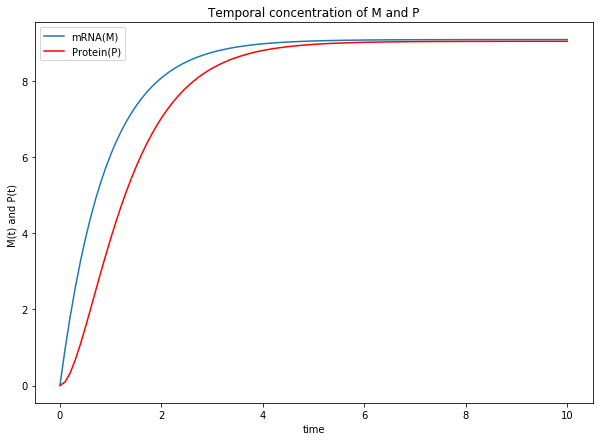
\includegraphics[scale=0.5]{./gaphics/q_8.png}
\caption{ }
\label{fig:8}
\end{figure}

\section*{Question 9}
When the cell makes a lot of R,  effectively blocking the promoter from further activity.
In  a scenario like this we utilize the differential equations  \eqref{eq:10}  and \eqref{eq:11} to model the system. 
In the case case where R inhibits the promoter from further activity, therefore,  $K$ and $K_d$ tend to be very large. mRNA  will be produced at a constant rate which is equal to the quantity not allowed by Repressor. 
We have plotted the curves this these scenarios below.
\begin{figure*}[th!]
    \centering
    \begin{subfigure}[t]{0.5\textwidth}
        \centering
        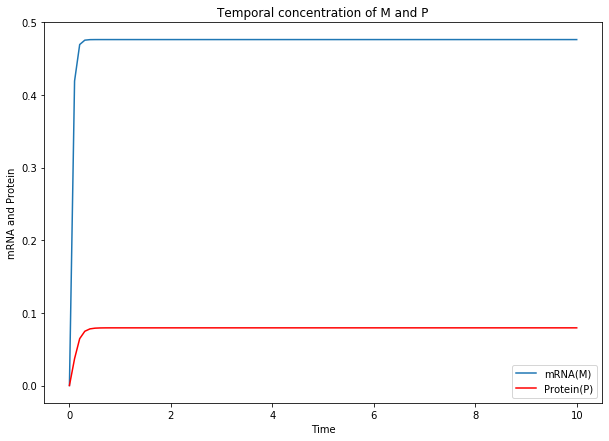
\includegraphics[height=1.8in]{./gaphics/q_9.png}
        %\caption{}
    \end{subfigure}%
    ~ 
    \begin{subfigure}[t]{0.5\textwidth}
        \centering
        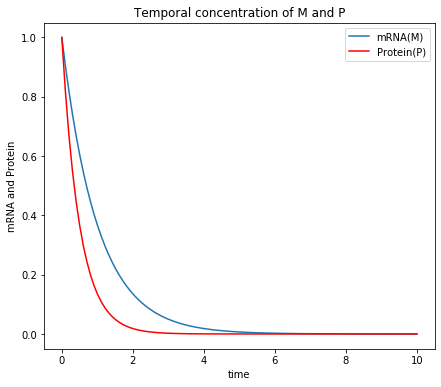
\includegraphics[height=1.8in]{./gaphics/q_9b.png}
        %\caption{}
    \end{subfigure}
    \caption{}
\end{figure*}

\section*{Question 10}
Considering a gene Y that has a binding site for activator A.  When there is no A,  gene Y
can be transcribed at a low level,  and when A is present,  it binds to gene Y and greatly
stimulates transcription.  The diagram of the gene and its promoter when it is not bound by A,
and another diagram when it is being bound by A is presented in Figure \ref{fig:10}.
\begin{figure*}[th!]
    \centering
    \begin{subfigure}[t]{0.5\textwidth}
        \centering
        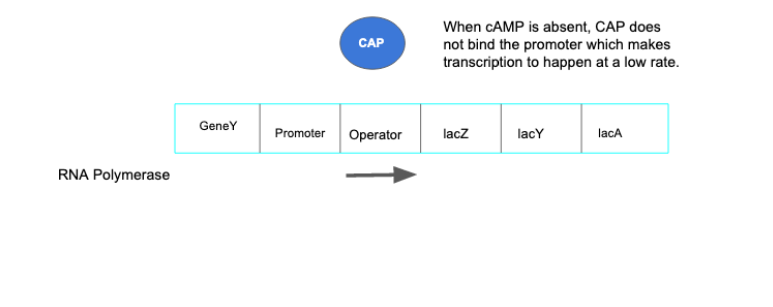
\includegraphics[height=1.8in]{./gaphics/q_10a.png}
        %\caption{}
    \end{subfigure}%
    ~ 
    \begin{subfigure}[t]{0.5\textwidth}
        \centering
        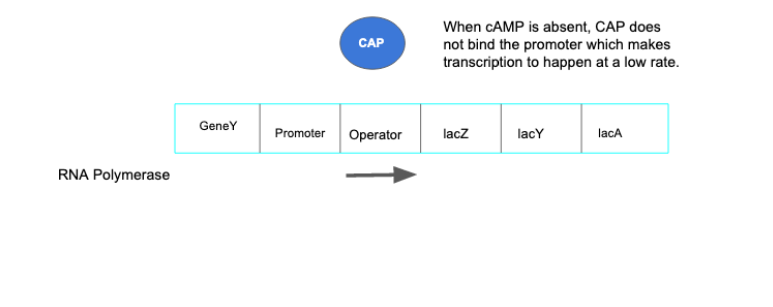
\includegraphics[height=1.8in]{./gaphics/q_10a.png}
        %\caption{}
    \end{subfigure}
    \caption{}
    \label{fig:10}
\end{figure*}

\section*{Question 11}
A derived model for the effect
of a sudden appearance of high levels of A on the steady state levels of gene Y mRNA and
protein is presented in the differential equations \eqref{eq:12}  and \eqref{eq:13}.
\begin{equation}
\frac{dM}{dt} =  \beta M -   \lambda M 
\label{eq:12}
\end{equation}
\begin{equation}
\frac{dP}{dt} =  \alpha M -   \gamma_p P 
\label{eq:13}
\end{equation}
The graph that shows effect
of a sudden appearance of high levels of A on the steady state levels of gene Y mRNA and
protein.
\begin{figure}[H]
\centering
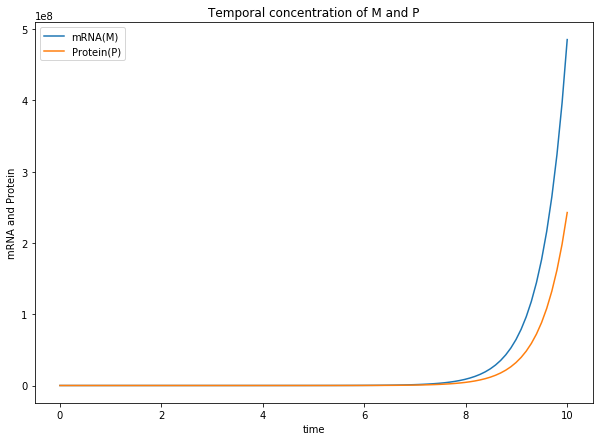
\includegraphics[scale=0.5]{./gaphics/q_11.png}
\caption{ }
\end{figure}
\end{document}